%--------------------------------------------------------------------------
% Methodology
%--------------------------------------------------------------------------

\chapter{Methodology}
\label{cha: methodology}

\section{Study area}
\label{sec: method-study-area}

The region of Northern Luzon, Philippines (approx. geographic coordinates: upper- left: 120$\,^{\circ}$ E, 18$\,^{\circ}$ N; lower-right: 123$\,^{\circ}$ E, 16$\,^{\circ}$ N) was chosen as an appropriate study area because all nine forest cover types based on the FAO FCCS were present in the region. The study area covers 16 provinces, either fully or partially, including: Abra, Apayao, Aurora, Benguet, Cagayan, Ifugao, Ilocos Norte, Ilocos Sur, Isabela, Kalinga, La Union, Mountain Province, Nueva Ecija, Nueva Vizcaya, Pangasinan, and Quirino (Fig. \ref{fig: method-fig3.1}). Northern Luzon experiences tropical cyclones very frequently, and spans three climate regimes based on the modified Coronas classification, particularly: Type I over Ilocos region (pronounced wet and dry season); Type III over Cagayan River Basin (short dry season with no pronounced maximum rain period); and Type IV over Northern Sierra Madre (no dry season and no pronounced maximum rain period).

The study area covers a total land area of 4.9 M ha, of which approximately 3.1 M ha (63\%) is comprised of non-forest land cover and 1.8M ha (37\%) is comprised of forest cover types based on the 2010 NAMRIA land cover map. Expansive agricultural areas are situated in the Cagayan Valley between the Cordilleras and Northern Sierra Madre ranges. Of the total land area of forest cover types, the majority is comprised of closed forest broadleaved (FCFB) at 38\%; open forest broadleaved (FOFB) at 46\%; open forest coniferous (FOFC) at 9\%; and the remaining 7\% by other forest cover types. A detailed tabulation of total land area of forest cover types per province is presented in Appendix 2.

\begin{figure}
	\centering
	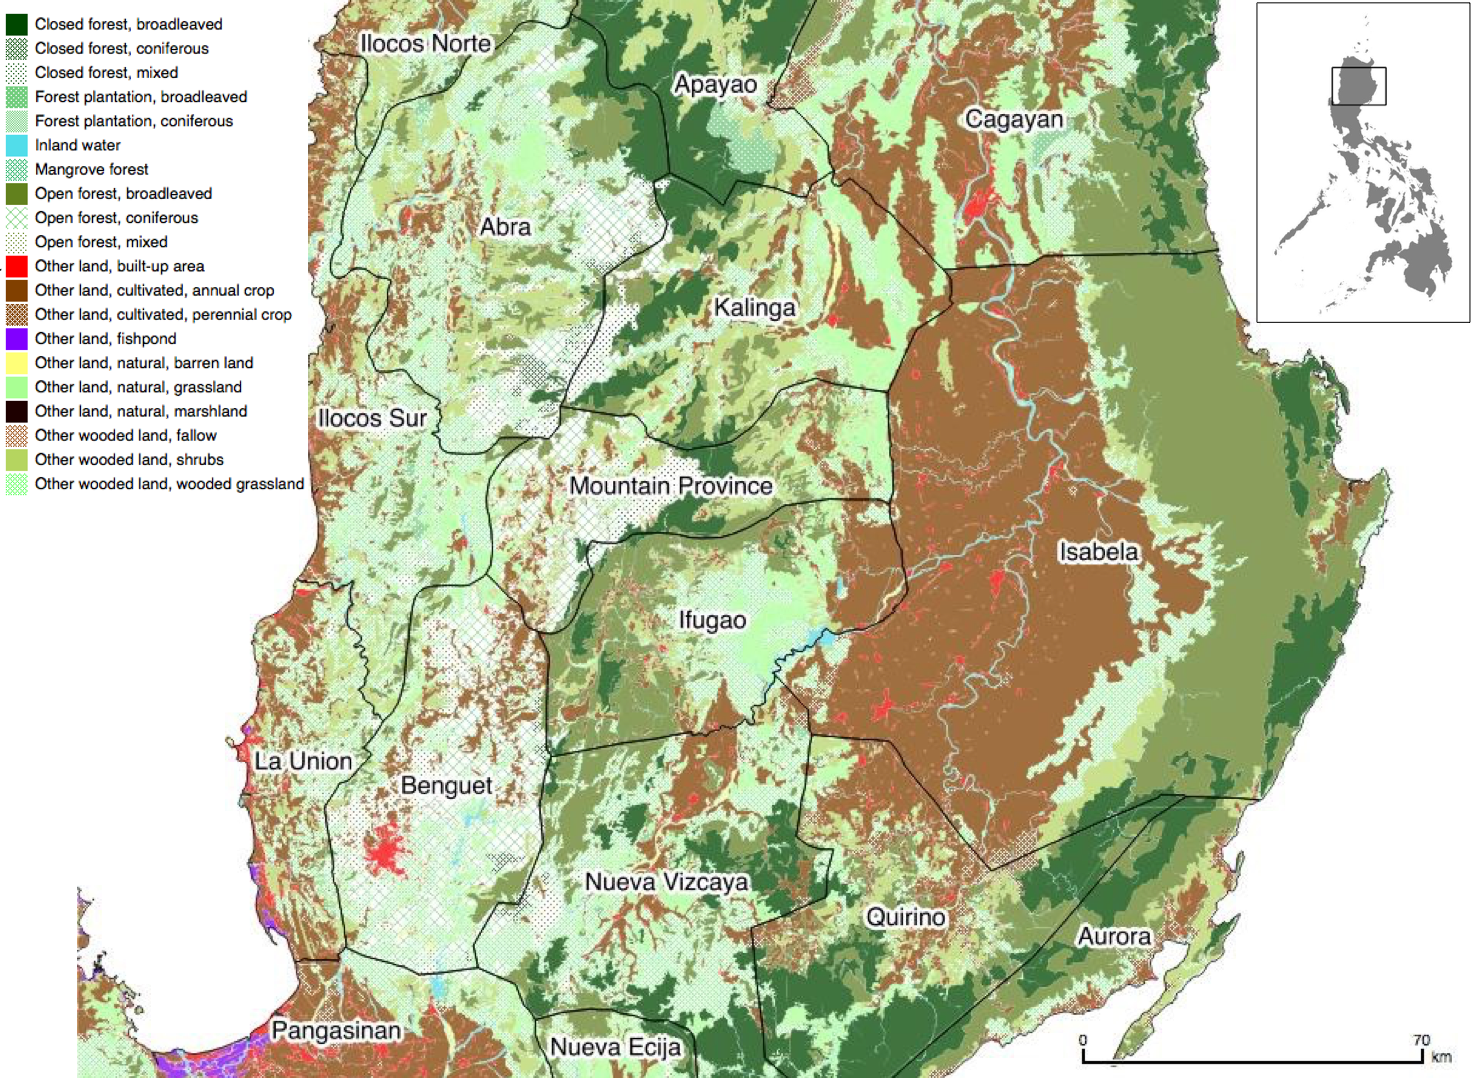
\includegraphics[width=1.0\textwidth]{fig_study-area.png}
	\caption[Study area in Northern Luzon, Philippines showing the 2010 land cover map based on NAMRIA data.]{Study area in Northern Luzon, Philippines showing the 2010 land cover map based on NAMRIA data.}
	\label{fig: method-fig3.1}
\end{figure}

\section{Data}
\label{sec: method-data}

For this study, the following datasets were used:

\begin{enumerate}
	\item Dual-polarised 25 m spatial resolution ALOS/PALSAR mosaic data (HH, HV) from JAXA through the K\&C Initiative (\cite{rosenqvist_initiating_2001}; \cite{rosenqvist_kyoto_2010}). The PALSAR mosaics, provided as 1x1 degree tiles, are radiometrically and geometrically calibrated large-scale datasets generated using JAXA's mosaicking algorithm, which consists of the pre-processing the long-strip PALSAR data; orthorectification and slope correction using a DEM; suppression of differences in intensity between neighbouring strips; and metadata preparation (e.g., dates of launch, local incidence angle, radar shadow, layover, and valid/invalid data) to support data interpretation (\cite{shimada_generating_2010}).
	Multi-year ALOS/PALSAR mosaic data (2007, 2008, 2009, 2010) were used to assess temporal consistency and suitability for periodic monitoring of forest cover. A total of 24 ALOS/PALSAR mosaic tiles were used with six tiles per year (i.e., 17N120E, 17N121E, 17N122E, 18N120E, 18N121E, 18N122E). All PALSAR tiles consist two channels, the HH and HV polarisation. The metadata layers, specifically the date of acquisition layer and the mask layer (for excluding radar shadow and layover pixels), corresponding to each mosaic tile per year were also used.
	\item Shuttle Radar Topography Mission (SRTM) elevation data product available from the United States Geological Survey. The SRTM DEM 1 arc-second (\url{~}30 m spatial resolution) global void-filled data was downloaded through the EarthExplorer portal. Nine DEM tiles were used (i.e., 16N120E, 16N121E, 16N122E, 17N120E, 17N121E, 17N122E, 18N120E, 18N121E, 18N122E).
	\item National 2010 NAMRIA land cover map. The data in vector format was accessed through the Forest Management Bureau. The land cover and forest type classes were based on the FAO GFRA categories (Table \ref{tab: intro-table2.1}) composed of a total of 20 land cover classes consisting of nine forest types.
\end{enumerate}

\section{Overall workflow}
\label{sec: method-overall-workflow}

The primary steps in the overall image processing workflow, which are discussed in the proceeding sub-sections, consists of image pre-processing (Sec. \ref{sec: method-preprocessing}), identification of regions of interest (Sec. \ref{sec: method-roi-identification}), image segmentation (Sec. \ref{sec: method-segmentation}), extraction of feature attributes and backscatter analysis (Sec. \ref{sec: method-feature-extraction}), hierarchical clustering (Sec. \ref{sec: method-clustering}), and decision tree classification and ruleset development (Sec. \ref{sec: method-decision-tree}). The overall workflow diagram shows the data used, intermediate outputs, processes implemented, and the final outputs (Fig. \ref{fig: method-fig3.2}).

\begin{figure}
	\centering
	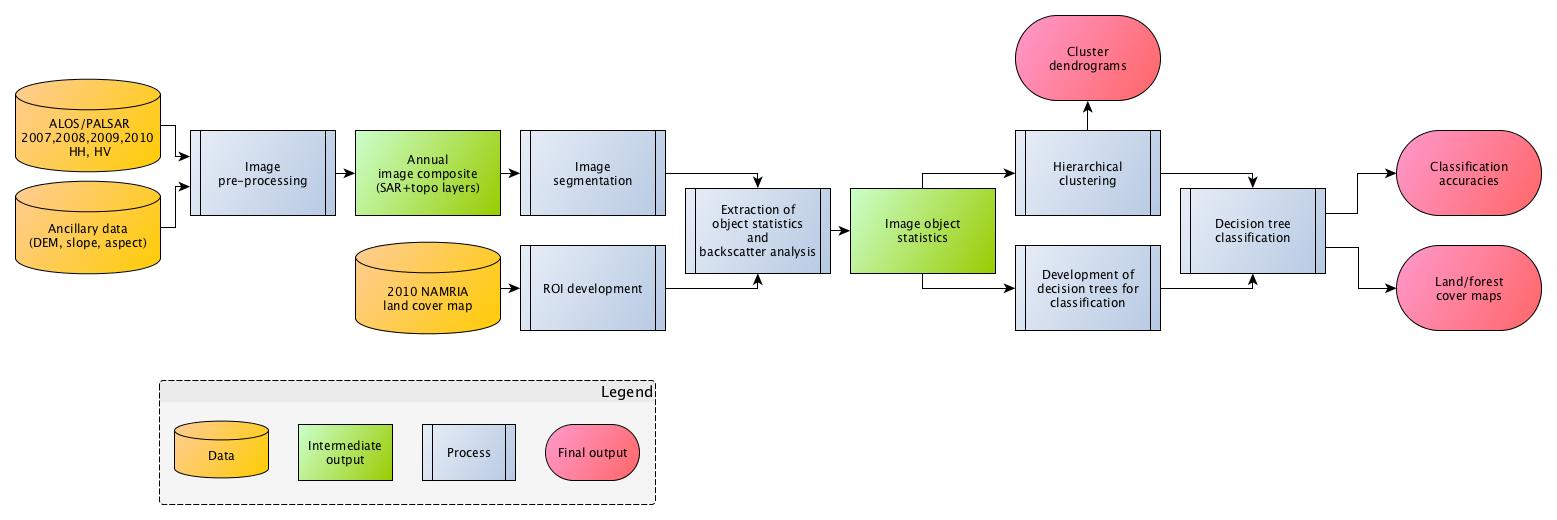
\includegraphics[width=1.0\textwidth]{fig_revised-methodology.jpg}
	\caption[Overall image processing workflow implemented in the study.]{Overall image processing workflow implemented in the study.}
	\label{fig: method-fig3.2}
\end{figure}

\section{Image pre-processing}
\label{sec: method-preprocessing}

Image pre-processing steps, which are presented as a sub-workflow diagram in Fig. \ref{fig: method-fig3.3}, were carried out in ENVI v.4.8 software (Exelis VIS, Inc. USA). For SAR data, each PALSAR data layer was mosaicked into a single regional image prior to geocoding and re-projection to UTM Zone 51 North coordinate system and WGS84 datum. The pixel dimensions of each image were 12844 columns x 8953 rows. To reduce signal noise from the radar data, a Lee filter was applied to preserve image sharpness and detail while suppressing speckle noise (\cite{lee_digital_1980}; \cite{lee_speckle_1981}), and with a small 5x5 kernel window to preserve texture information (\cite{lee_speckle_1994}). After minimising the speckles, ratio images (HH/HV) were generated using the HH and HV regional mosaics for each year. Then, HH and HV polarisation images were converted from amplitude to normalised radar cross-section, or sigma-nought ($\sigma$\textsuperscript{0}; units in dB) using Eq. \ref{eqn: method-eq1}:

\begin{equation} \label{eqn: method-eq1}
		\sigma^0=10\cdot log\textsubscript{10}[DN^2]+CF
\end{equation}

\noindent Where \textit{DN} is the digital number and \textit{CF} is the calibration factor with a value of –83.0 dB for ALOS/PALSAR data (\cite{rosenqvist_alos_2007}). A masking process was implemented on the PALSAR regional mosaics using the corresponding mask layers for each year to exclude unwanted pixels affected by shadow and layover in the radar data.

For the topographic data, the SRTM DEM tiles were mosaicked together prior to re- projection to UTM Zone 51 North WGS84, and subsequently resampled to 25 m spatial resolution and cropped to match the extents and dimensions of the SAR mosaic images. The slope and aspect layers were subsequently computed from the mosaicked DEM. Lower kernel sizes (i.e., 3x3, 5x5, and 7x7) were initially tested but the resulting models contained artifacts; hence, a 9x9 kernel size was used to generate the final slope (in percent) and aspect models.

\begin{figure}
	\centering
	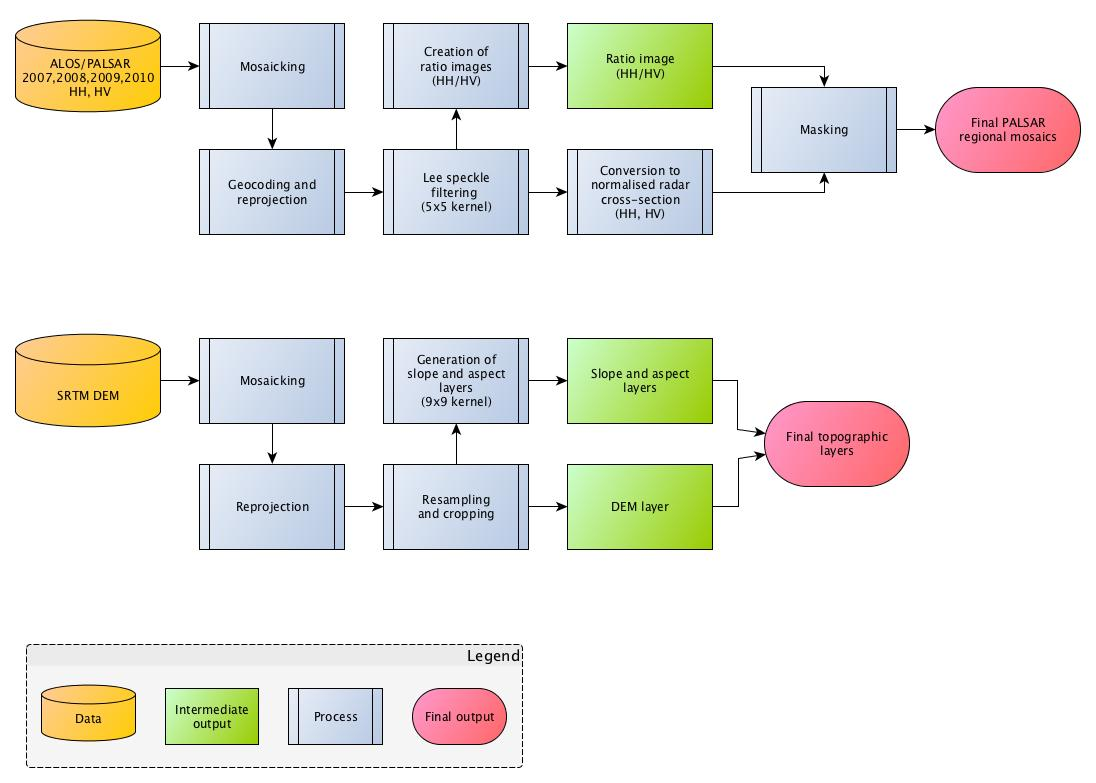
\includegraphics[width=1.0\textwidth]{fig_image-preprocessing.jpg}
	\caption[Detailed sub-workflow for image pre-processing steps implemented on SAR and topographic datasets.]{Detailed sub-workflow for image pre-processing steps implemented on SAR and topographic datasets.}
	\label{fig: method-fig3.3}
\end{figure}

\section{Design of a multi-level classification hierarchy}
\label{sec: method-class-hierarchy}

A multi-level land cover classification hierarchy was designed to guide the selection of regions of interest (ROI) and the decision tree classification (Fig. \ref{fig: method-fig3.4}). The first three levels were designed to classify the image into broad-level classes and extract the Forest class. Within the Forest class, after setting aside all Non-Forest class, the class hierarchy of subsequent levels was defined based on the result of the hierarchical clustering.

Starting with the entire image dataset, each level bifurcated into two classes and carried out sequentially one level after another. At Level 1, the data was split into either Land or Water classes. Then at Level 2, Water classes were set aside, and the Land class was assigned into either Vegetation or Non-Vegetation classes. At Level 3, the Vegetation class was split into either Forest or Non-Forest classes while the Non- Vegetation class was set aside. At Level 4, the splitting into forest types was carried out following the dendrograms resulting from the hierarchical cluster analysis.

\begin{figure}
	\centering
	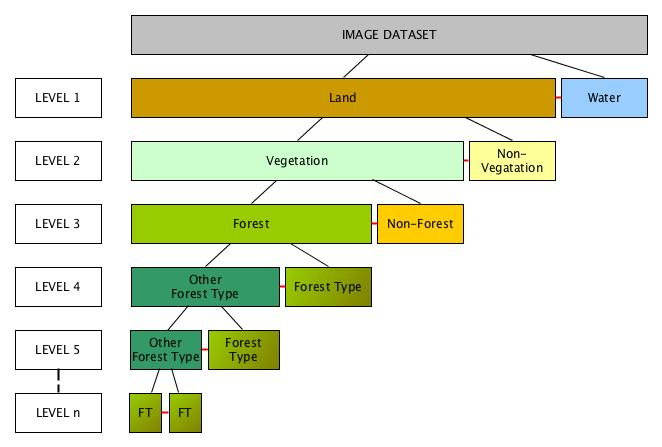
\includegraphics[width=1.0\textwidth]{fig_classification-hierarchy.jpg}
	\caption[The classification hierarchy proposed for this study.]{The classification hierarchy proposed for this study (note: FT is Forest Type).}
	\label{fig: method-fig3.4}
\end{figure}

\section{Identification of regions of interest}
\label{sec: method-roi-identification}

The identification of the ROIs was carried out in Quantum GIS v.2.12 software (QGIS Project Team). Prior to delineating ROIs, the detailed land cover classes were grouped into broad-level classes based on the multi-level classification hierarchy (Fig. \ref{fig: method-fig3.4}; Table \ref{tab: method-table3.1}). To aid in identifying and delineating the ROIs, the 2010 NAMRIA land cover map was used as a base map. The PALSAR mosaics were also visually inspected during the delineation of each ROI before assigning it to a specific class and to ensure a 5x5 kernel size polygon. Other ancillary vector data were also used to aid in identifying the ROIs, including OpenStreetMap data such as roads, buildings, and rivers (\cite{geofabrik_gmbh_philippines_2015}); and the Landsat-based 2010 mangrove map of the Philippines developed by Long et al. \citeyearpar{long_mapping_2013} to aid in identifying regions of interest in mangrove forests. A total of 1,451 ROIs were identified representing the land cover classes, and each ROI record reflected the multi-level classification hierarchy in the attribute table (Table \ref{tab: method-table3.1}). The distribution of the ROIs selected over the study area is shown in Fig. \ref{fig: method-fig3.5}.\\

\begin{spacing}{1.0}
\begin{longtable}[h!]{ p{1.4cm} p{1.8cm} p{1.4cm} p{6.9cm} p{1.5cm} }

    \caption[Hierarchy and grouping of land cover from detailed to broad-level classes.]{Hierarchy and grouping of detailed land cover classes into broad-level classes.}
    \label{tab: method-table3.1}\\
    
    	\toprule
    	Level 1 & Level 2 & Level 3 & 2010 NAMRIA Land Cover Classes & Number of ROIs\\ 
    	\midrule
    	\endhead
    	
		Land & Vegetation & Forest & Closed forest, broadleaved (FCFB) & 100\\
		{} & {} & {} & Closed forest, coniferous (FCFC) & 100\\
		{} & {} & {} & Closed forest, mixed (FCFM) & 100\\
		{} & {} & {} & Open forest, broadleaved (FOFB) & 186\\
		{} & {} & {} & Open forest, coniferous (FOFC) & 101\\
		{} & {} & {} & Open forest, mixed (FOFM) & 100\\
		{} & {} & {} & Forest plantation, broadleaved (FFPB) & 90\\
		{} & {} & {} & Forest plantation, coniferous (FFPC) & 30\\
		{} & {} & {} & Mangrove forest (LVMG) & 48\\[2pt]
		\cmidrule{3-5}
		{} & {} & Non- & Other wooded land, shrubs & 317\\
		{} & {} & Forest & Other wooded land, wooded grassland & {}\\
		{} & {} & {} & Other land, grassland & {}\\
		{} & {} & {} & Other land, annual crop & {}\\
		{} & {} & {} & Other land, perennial crop & {}\\[5pt]
		\cmidrule{2-5}
		{} & Non- & {} & Other wooded land, fallow & 67\\
		{} & Vegetation & {} & Other land, built-up area & {}\\
		{} & {} & {} & Other land, barren land & {}\\[5pt]
		\cmidrule{1-5}
		Water & {} & {} & Inland water & 212\\
		{} & {} & {} & Fishpond & {}\\
		\bottomrule
    
\end{longtable}
\end{spacing}

\begin{figure}
	\centering
	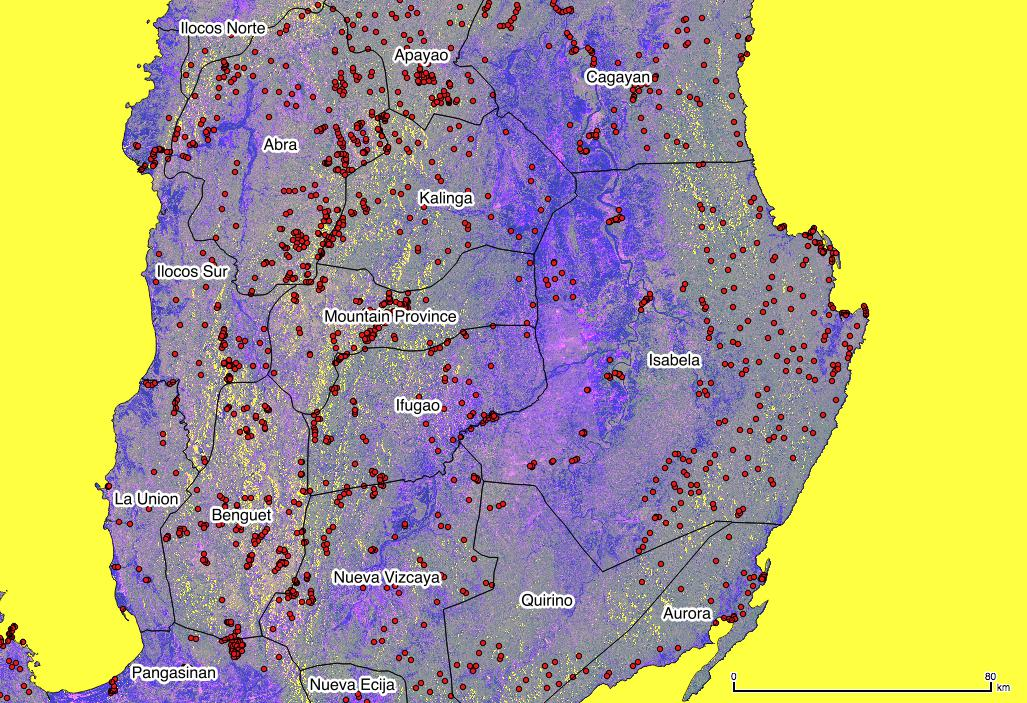
\includegraphics[width=1.0\textwidth]{fig_roi-locations.jpg}
	\caption[The distribution of the regions of interest selected over the study area in Northern Luzon, Philippines.]{The distribution of the regions of interest (red points) selected over the study area in Northern Luzon, Philippines. The 2010 PALSAR mosaic image is shown in the background.}
	\label{fig: method-fig3.5}
\end{figure}

\section{Image segmentation}
\label{sec: method-segmentation}

Image segmentation was implemented in eCognition Developer v.8.9 software (Trimble Germany GmbH). The segmentation method that is implemented in eCognition is an iterative process that minimises the average heterogeneity of generated segments (\cite{baatz_multi-resolution_2000}). The measure of heterogeneity consists of a spectral and spatial component (\cite{benz_multi-resolution_2004}; \cite{happ_multi-resolution_2010}). Spectral heterogeneity is defined on the values of the spectral responses of the pixels within the segments. Spatial heterogeneity is based on two shape attributes: smoothness and compactness of the segments. Another parameter, scale, is the stopping criterion for the optimisation process. Prior to fusion of two adjacent objects, the resulting increase in heterogeneity is computed such that if the resulting increase exceeds a threshold determined by the scale parameter then no further fusion takes place and the segmentation stops (\cite{benz_multi-resolution_2004}). A merge with a better degree of fitting (i.e., smaller value) than the scale parameter fulfils the homogeneity criterion (\cite{baatz_multi-resolution_2000}). Hence, the larger the scale parameter, the more objects can be fused and the larger the segments grow (\cite{baatz_multi-resolution_2000}).

The input data for segmentation consisted of the set of images, including the 12 ALOS/PALSAR data layers (i.e., HH and HV polarisation and HH/HV ratio images for each year) and 3 topographic data layers (i.e, elevation, slope, and aspect), totalling 15 input image layers. To determine the values of the parameters to be used for image segmentation procedure, different values were tested on each parameter to see whether the resulting segments made an acceptable delineation of image features (Appendix 3.). For multi-resolution segmentation, the user sets the following parameters: scale, shape, compactness, and image weights. The values of 5, 10, and 20 were tested for the scale parameter. For shape and compactness, the values of 0.1, 0.5, and 0.9 were used for each parameter, thereby testing nine combinations of values between shape and compactness (i.e., 0.1-0.1; 0.1- 0.5; 0.1-0.9; 0.5-0.1; 0.5-0.5; 0.5-0.9; 0.9-0.1; 0.9-0.5; and 0.9-0.9). For image weights, a value of 1 was used uniformly on all layers, both for the SAR and topographic layers.

After a visual assessment of the segmentation tests, a scale parameter value of 10 was chosen since a value of 5 was too detailed and a value of 20 had generalised small features. Next, a shape value of 0.1 and a compactness value of 0.9 were selected since the segments closely followed the form of image features. For image weights, a value of 1 was retained for SAR data layers only. Topographic layers were given image weight values of 0 since they introduced regular-shaped rectangular segments that were not capturing the form of image features. The final values chosen for the multi-resolution segmentation parameters were: scale = 10; shape = 0.1; compactness = 0.9; image weights = 1 for SAR layers and 0 for topographic layers (Appendix 3). The total number of segments delineated for each PALSAR regional mosaic were as follows: 2007 = 182,876 segments; 2008 = 184,917 segments; 2009 = 186,369 segments; 2010 = 191,588 segments.

\section{Extraction of feature attributes and backscatter analysis}
\label{sec: method-feature-extraction}

Object-level feature attributes were computed for all the delineated land cover ROIs in eCognition software. Feature attributes were calculated, particularly the mean and standard deviation, both from the yearly PALSAR regional mosaics and topographic layers; and eight GLCM measures from each of the PALSAR data layers. The GLCM texture measures include angular second moment, contrast, correlation, dissimilarity, entropy, homogeneity, mean, and standard deviation (variance). Thirty feature attributes were extracted from the SAR data layers per year (including polarisation and texture attributes) and 6 attributes from the topographic layers (Table \ref{tab: method-table3.2}). Tabular databases were generated containing these feature attributes such that four tables were produced, each corresponding to the attributes per annual PALSAR regional mosaics plus the topographic layer attributes. These tabular databases were then used as inputs for subsequent backscatter analysis, the hierarchical clustering, and the decision tree classification in R statistical software (\cite{r_core_team_r:_2016}).\\

\begin{spacing}{1.0}
\begin{longtable}[h!]{ p{2.6cm} p{2.6cm} p{2.6cm} p{2.6cm} p{2.6cm} }

    \caption[Object-level feature attributes extracted from the images.]{Object-level feature attributes extracted from the images.}
    \label{tab: method-table3.2}\\
    
    	\toprule
    	Polarisation & Topographic & {} & Texture & {}\\
    	\cmidrule{3-5}
    	{} & {} & GLCM HH & GLCM HV & GLCM HH/HV\\
    	\midrule
    	\endhead
    	
		Mean HH & Mean DEM & Ang. 2$^{nd}$ Mom & Ang. 2$^{nd}$ Mom & Ang. 2$^{nd}$ Mom\\
		Mean HV & Mean Slope & Contrast & Contrast & Contrast\\
		Mean HH/HV & Mean Aspect & Correlation & Correlation & Correlation\\
		SD HH & SD DEM & Dissimilarity & Dissimilarity & Dissimilarity\\
		SD HV & SD Slope & Entropy & Entropy & Entropy\\
		SD HH/HV & SD Aspect & Homogeneity & Homogeneity & Homogeneity\\
		{} & {} & Mean & Mean & Mean\\
		{} & {} & SD & SD & SD\\
		
		\bottomrule
    
\end{longtable}

	\noindent Note: HH, horizontal transmit - horizontal receive; HV, horizontal transmit - vertical receive; GLCM, grey level co-occurrence matrix; DEM, digital elevation model; SD, standard deviation.\\ \newline

\end{spacing}

PALSAR mosaic data are comprised of strip (or path) data acquired on different dates that are pre-processed and mosaicked together as end-user products (Fig. \ref{fig: method-fig3.6}; \cite{shimada_generating_2010}). The strip data comprising one annual regional PALSAR mosaic were acquired over different seasons/dates. Also, the strip data along the same path acquired over the same locality were acquired over different years for the annual mosaics. To assess the temporal consistency of the PALSAR mosaic data, a radar backscatter analysis of forest cover types was done for PALSAR mosaics, first, across adjacent strips within a single acquisition year; and second, within the same strip across multiple acquisition years. Box-whisker plots were generated using the \textit{ggplot2} package in R software (\cite{wickham_ggplot2:_2015}) to analyse the backscatter values of different forest types over the different dates of acquisition of the images.\\

\begin{figure}[!ht] \centering
	\captionsetup[subfigure]{width=2.0in} % <-- Use this to control text which is poorly spaced under a subfigure. 
	\begin{subfigure}[t]{0.49\textwidth}
		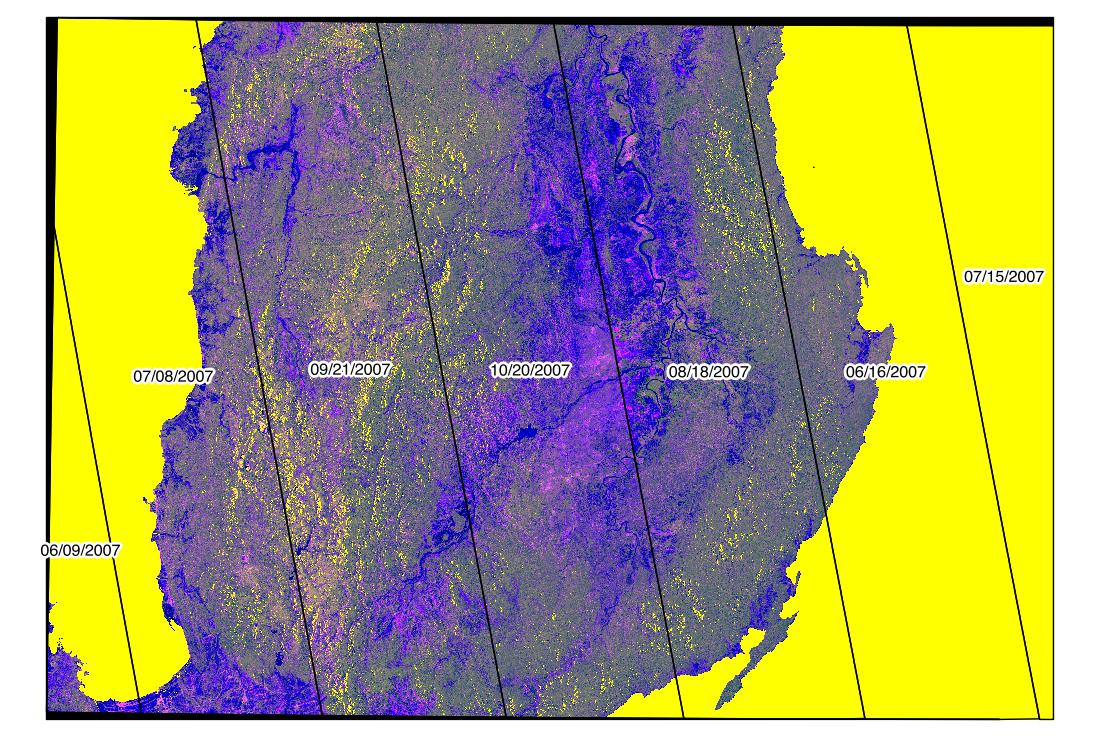
\includegraphics[width=\textwidth]{fig_palsar-2007-dates.jpg}
		\caption[Annual PALSAR mosaics.]{2007}
		\label{fig: method-fig3.6a}
	\end{subfigure}
	\begin{subfigure}[t]{0.49\textwidth}
		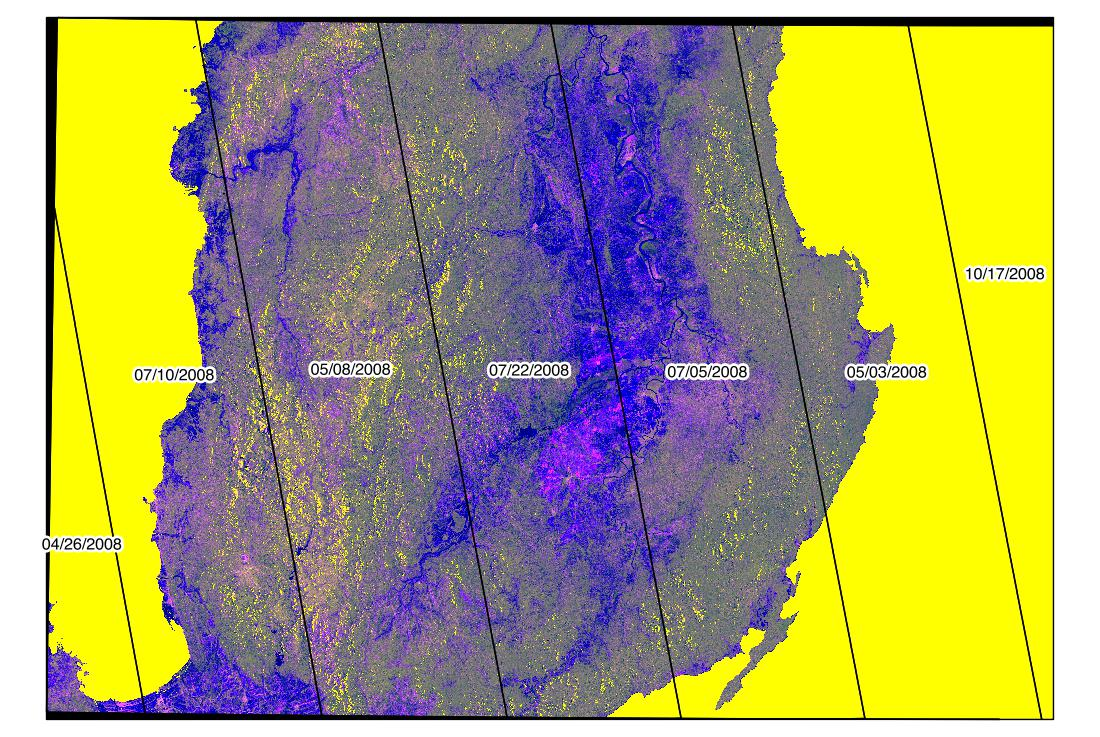
\includegraphics[width=\textwidth]{fig_palsar-2008-dates.jpg}
		\caption[Annual PALSAR mosaics.]{2008}
		\label{fig: method-fig3.6b}
	\end{subfigure}\\
	\vspace{10pt}
	\begin{subfigure}[t]{0.49\textwidth}
		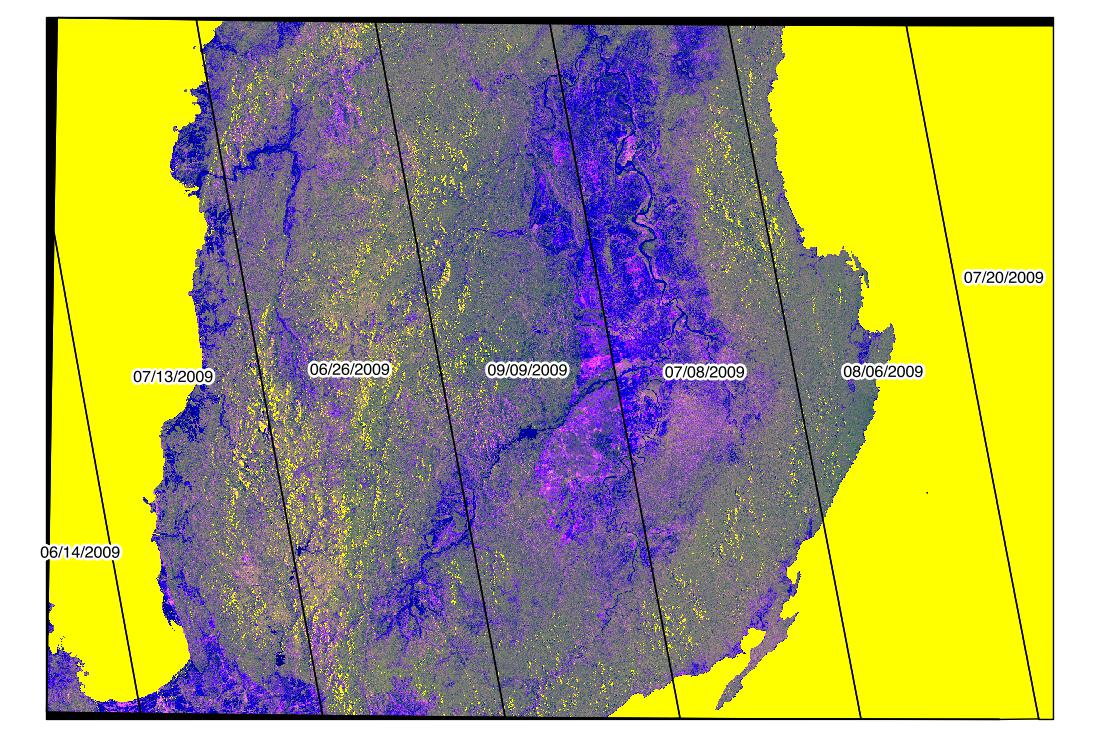
\includegraphics[width=\textwidth]{fig_palsar-2009-dates.jpg}
		\caption[Annual PALSAR mosaics.]{2009}
		\label{fig: method-fig3.6c}
	\end{subfigure}
	\begin{subfigure}[t]{0.49\textwidth}
		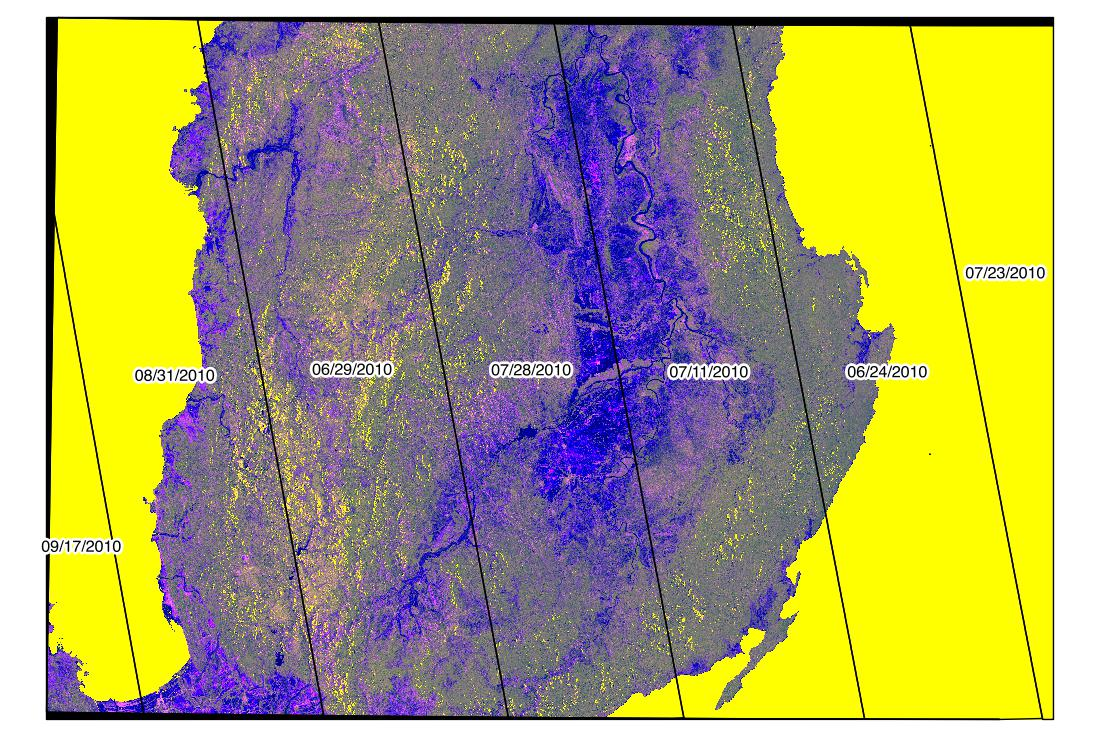
\includegraphics[width=\textwidth]{fig_palsar-2010-dates.jpg}
		\caption[Annual PALSAR mosaics.]{2010}
		\label{fig: method-fig3.6d}
	\end{subfigure}
	\caption[The annual PALSAR mosaics of Northern Luzon acquired in 2007, 2008, 2009, and 2010.]{The annual PALSAR mosaics of Northern Luzon acquired in (a) 2007, (b) 2008, (c) 2009, and (d) 2010. The extent of each strip (or path) data and the dates of acquisition of each strip are shown for each annual mosaic.}
	\label{fig: method-fig3.6}
\end{figure}

\section{Hierarchical clustering}
\label{sec: method-clustering}

Agglomerative hierarchical clustering was implemented using the \textit{pvclust} package in R software (\cite{suzuki_pvclust:_2006}; \cite{suzuki_pvclust:_2014}) with the tabular databases for each year as inputs. Both the temporal consistency of the multi-year SAR data and the cluster hierarchy of forest types were evaluated using the dendrograms. The \textit{pvclust} package was useful to assess the uncertainty or stability in hierarchical cluster analysis by calculating probability values (\cite{suzuki_pvclust:_2014}). An approximately unbiased (AU) p-value $\geq$ 0.95 indicates consistent or stable clustering/grouping and is strongly supported by the data.\\

\begin{spacing}{1.0}
\begin{longtable}[h!]{ p{2cm} p{2cm} p{9cm} }

    \caption[Four cases representing combinations of object-level feature attributes.]{The four cases representing combinations of object-level feature attributes.}
    \label{tab: method-table3.3}\\
    
    	\toprule
    	Case & Number of variables & Combinations of object-level feature attributes\\
       	\midrule
    	\endhead
    	
		1 & 6 & Polarisation\\
		2 & 12 & Polarisation + Topographic\\
		3 & 30 & Polarisation + Texture\\
		4 & 36 & Polarisation + Topographic + Texture\\
		
		\bottomrule \\
    
\end{longtable}
\end{spacing}

Four cases representing combinations of object-level feature attributes were used in evaluating the temporal consistency of the cluster hierarchy of forest types (Table \ref{tab: method-table3.3}). Hierarchical clustering was applied across the four cases with each case involving the four annual PALSAR mosaics. For Case 1, only the Polarisation feature attributes were evaluated. For Case 2, the Polarisation and Topographic feature attributes were evaluated. For Case 3, the Polarisation and Texture feature attributes were evaluated. Finally, for Case 4, the all feature attributes were evaluated.

In any case, consistency of the cluster hierarchy means that the hierarchical structure of the dendrogram does not change and the order and location of the nodes represented by forest types do not vary. The consistency of dendrograms was assessed through pairwise comparisons of dendrograms, totalling six pairs in each case. Baker's Gamma Indices were computed using the \textit{dendextend} package in R software (\cite{galili_dendextend:_2015}; \cite{galili_dendextend:_2015-1}) for comparing clustering dendrograms. The Baker’s Gamma Index (referred to as $\beta$ coefficient from here on) is a measure of association (similarity) between two dendrograms of hierarchical clustering (\cite{baker_stability_1974}). It is defined as a rank correlation between the stages at which pairs of objects combine in each of the two dendrograms (\cite{fowlkes_method_1983}). A Spearman's correlation is computed and the values can range between -1 to 1 with near 0 values meaning that the two dendrograms are not statistically similar (\cite{galili_dendextend:_2015}). The Baker's Gamma Indices for pairwise comparison of dendrograms for all cases were summarised and ranked to determine which case (or combination of feature attributes) gave the higher similarity between dendrograms.

\section{Decision tree classification and ruleset development}
\label{sec: method-decision-tree}

A decision tree classification approach using the \textit{tree} package in R software (Ripley, 2015), which is based on the CART algorithm by Breiman et al. (1984), was used to construct decision tree models. The tabular databases were used as the inputs for decision tree classification, designating the feature attributes as predictor variables and assigning classes depending on the classification level. At Level 1 classification, all objects were assigned into either Land or Water classes. Then at Level 2, Water classes were set aside, and only objects classified as Land from Level 1 were subsequently assigned into either Vegetation or Non-Vegetation classes. At Level 3, only objects classified as Vegetation from Level 2 are assigned into either Forest or Non-Forest classes while setting aside Non-Vegetation classes. In subsequent classification levels, forest cover types were classified one by one based the results of the hierarchical clustering until all forest cover types were classified.

Decision tree models were developed based on four cases or combinations of feature attributes to determine whether ancillary feature attributes (i.e., topographic, texture), in addition to polarisation, contribute to improving the classification accuracy of forest cover types. All decision trees were pruned using k-fold cross-validation to prevent overfitting. The case yielding the lowest misclassification error rates was selected and used as the basis for generating classification trees for each level for each year. A total of 44 classification trees were generated consisting of 11 trees in each year. The decision tree models produced in R software were translated as the bases for constructing the multi-level classification rulesets to produce forest cover maps in eCognition software.

An additional assessment of classification accuracies was done to discriminate closed and open canopy forests without following the hierarchical clustering result. The first three classification levels were maintained. At Level 4, mangrove forest (LVMG) was separated from all other forest types. For the final classification at Level 5, closed and open canopy forests were separated. Closed canopy forests included: closed broadleaved (FCFB), closed coniferous (FCFC), and closed mixed (FCFM). Open canopy forests included: open broadleaved (FOFB), open coniferous (FOFC), open mixed (FOFM), broadleaved forest plantation (FFPB), and coniferous forest plantation (FFPC).
